

\chapter{Supplementary figures}
\label{Supplementary figures}
\begin{figure}[htbp]
  \centering
  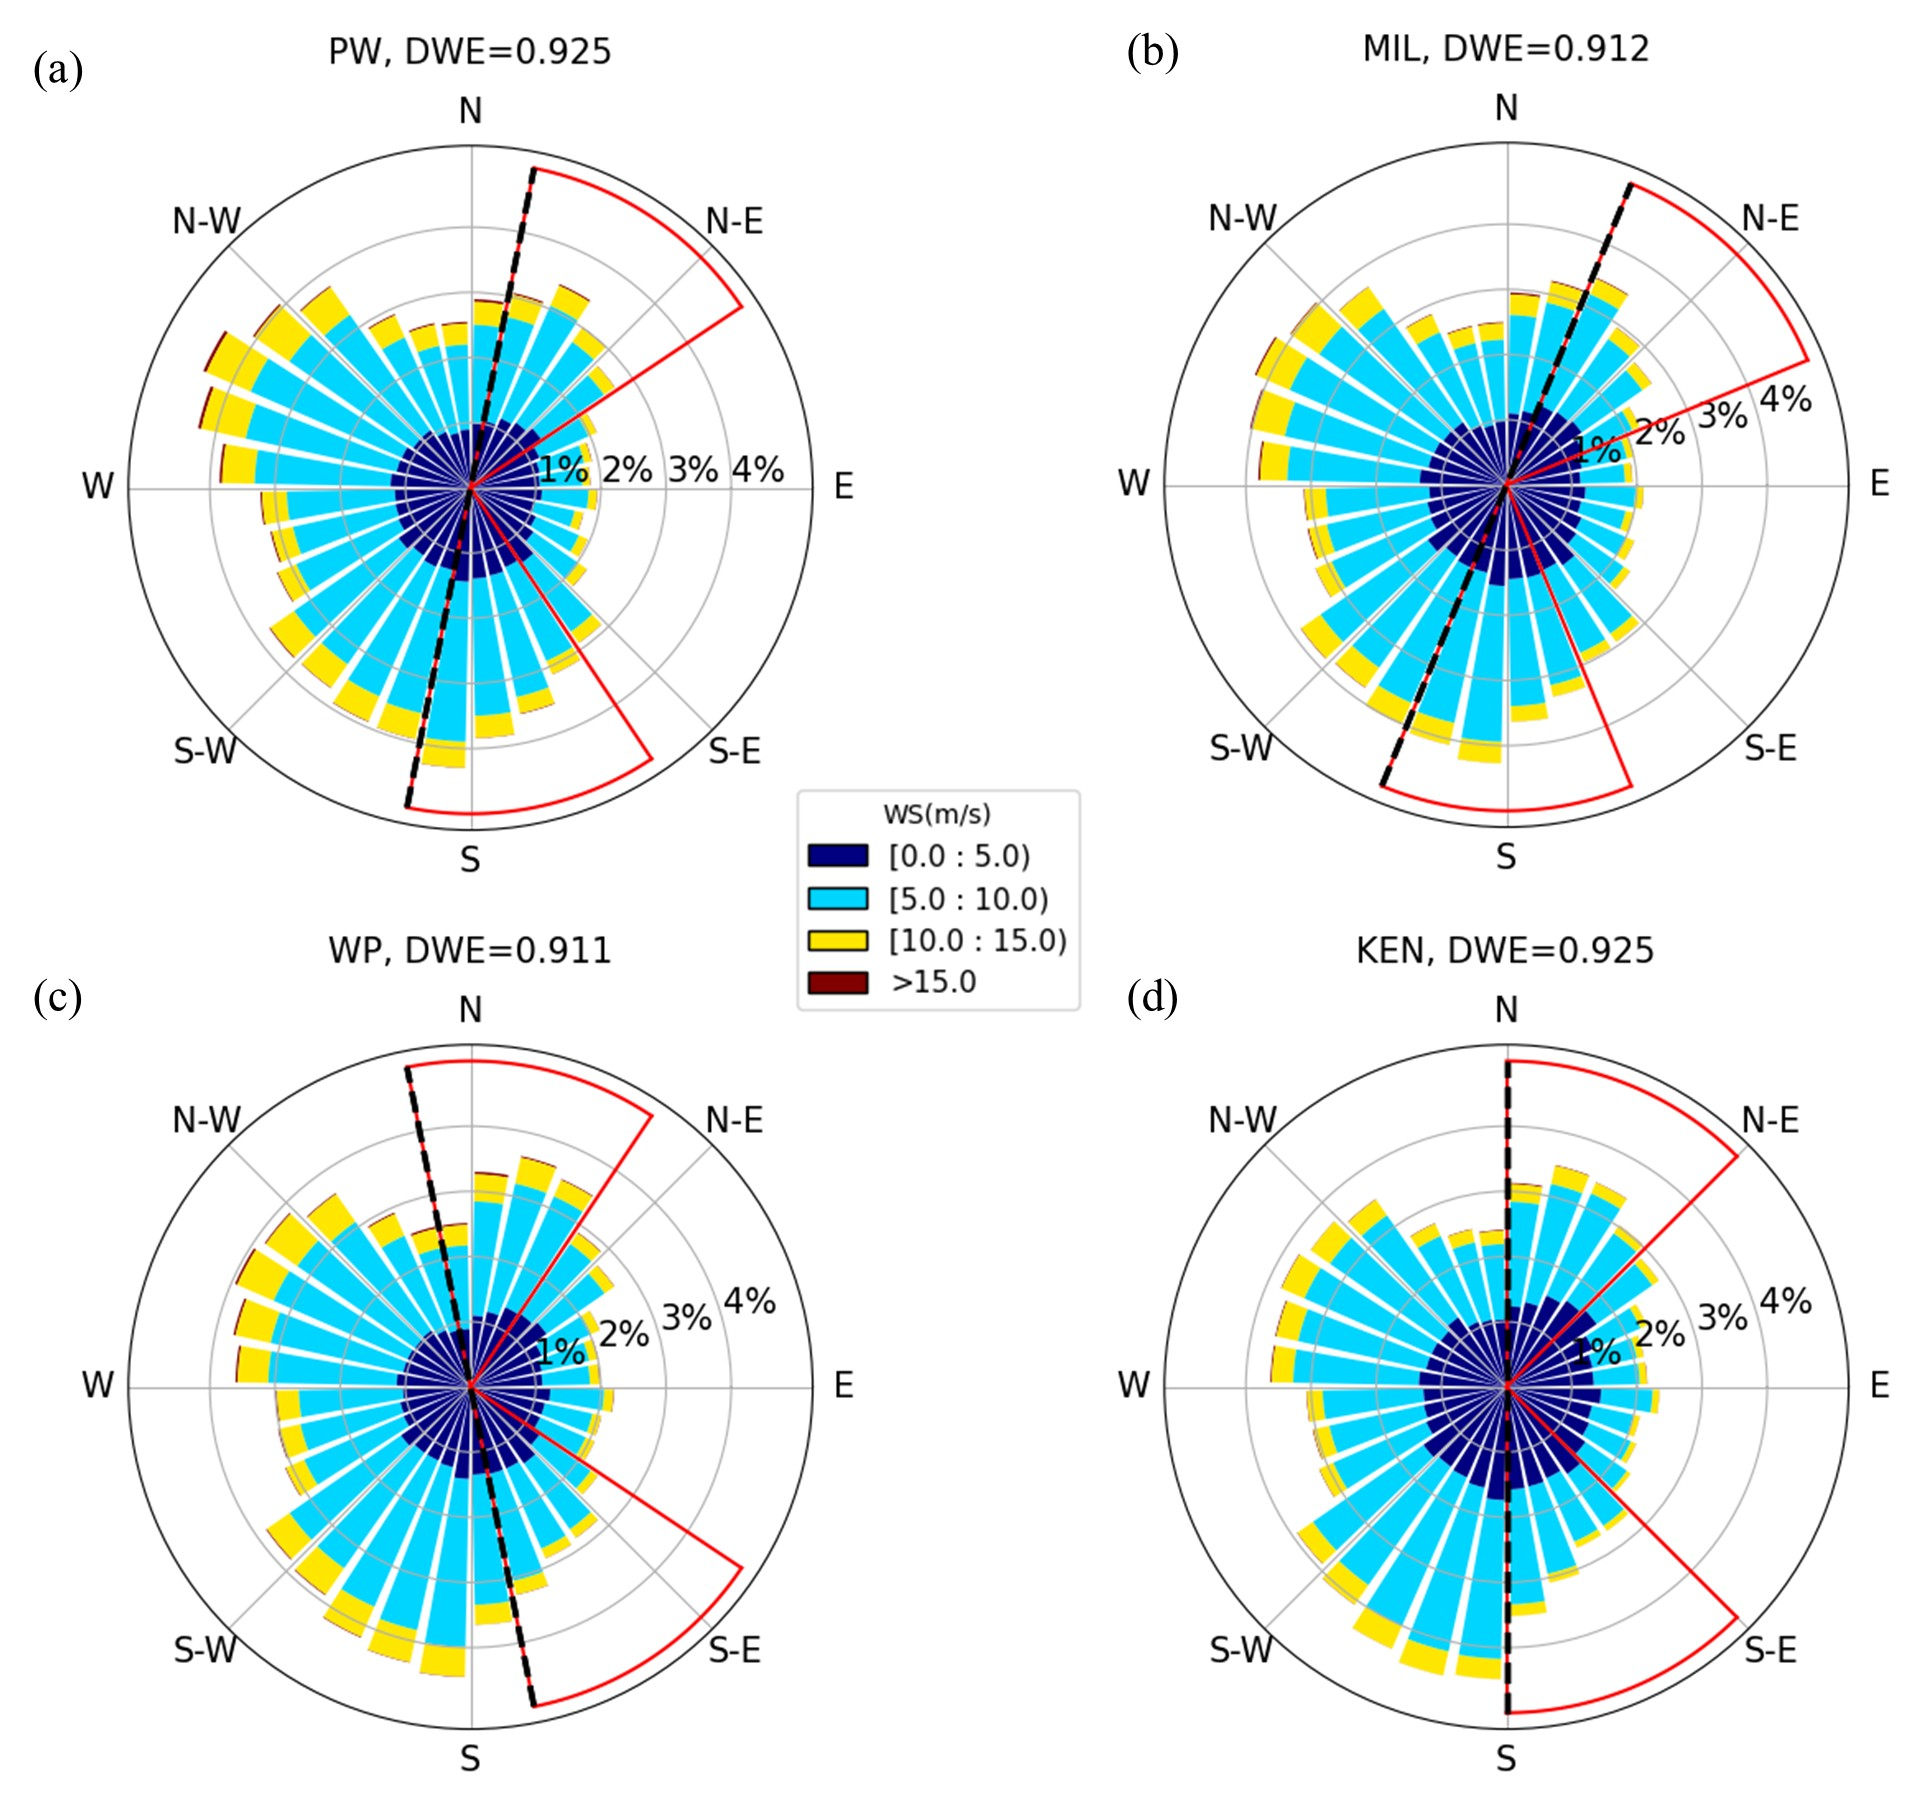
\includegraphics[width=0.8\textwidth]{appendix/resources/figure3-1a.jpg}
  \caption{Wind rose maps and DWE at 4 selected locations. (a) PW-Port Washington, (b) MIL-Milwaukee Harbor, (c) WP-Wind Point, and (d) KEN-Kenosha Harbor with their directional wave (wind) entropy.}
  \label{fig:fig3.1a}
\end{figure}

\begin{figure}[htbp]
  \centering
  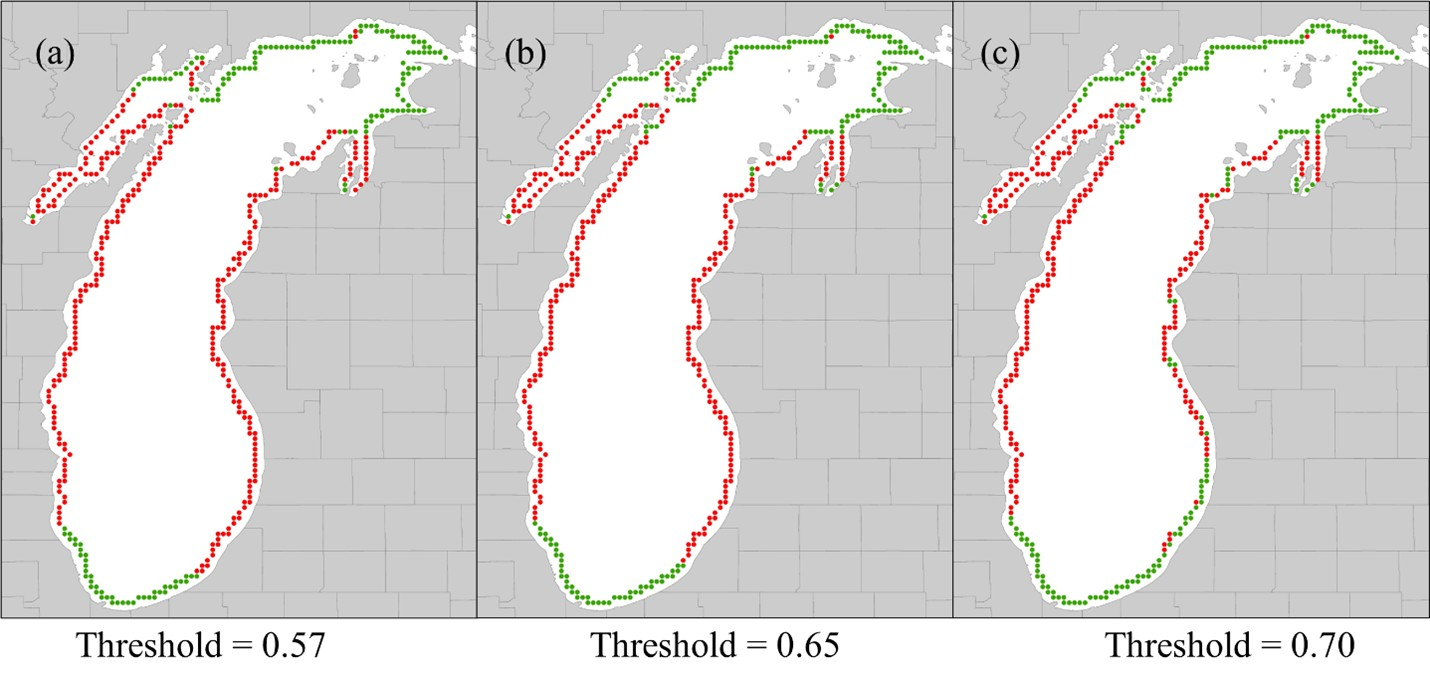
\includegraphics[width=0.8\textwidth]{appendix/resources/figure3-2a.jpg}
  \caption{Wave directionality in Lake Michigan for different DWE thresholds. Wave directionality (red dots are bi-directional and green dots are uni-directional) under three different thresholds: (a) 0.57 (b) 0.65 (c) 0.70.}
  \label{fig:fig3.2a}
\end{figure}

\begin{figure}[htbp]
  \centering
  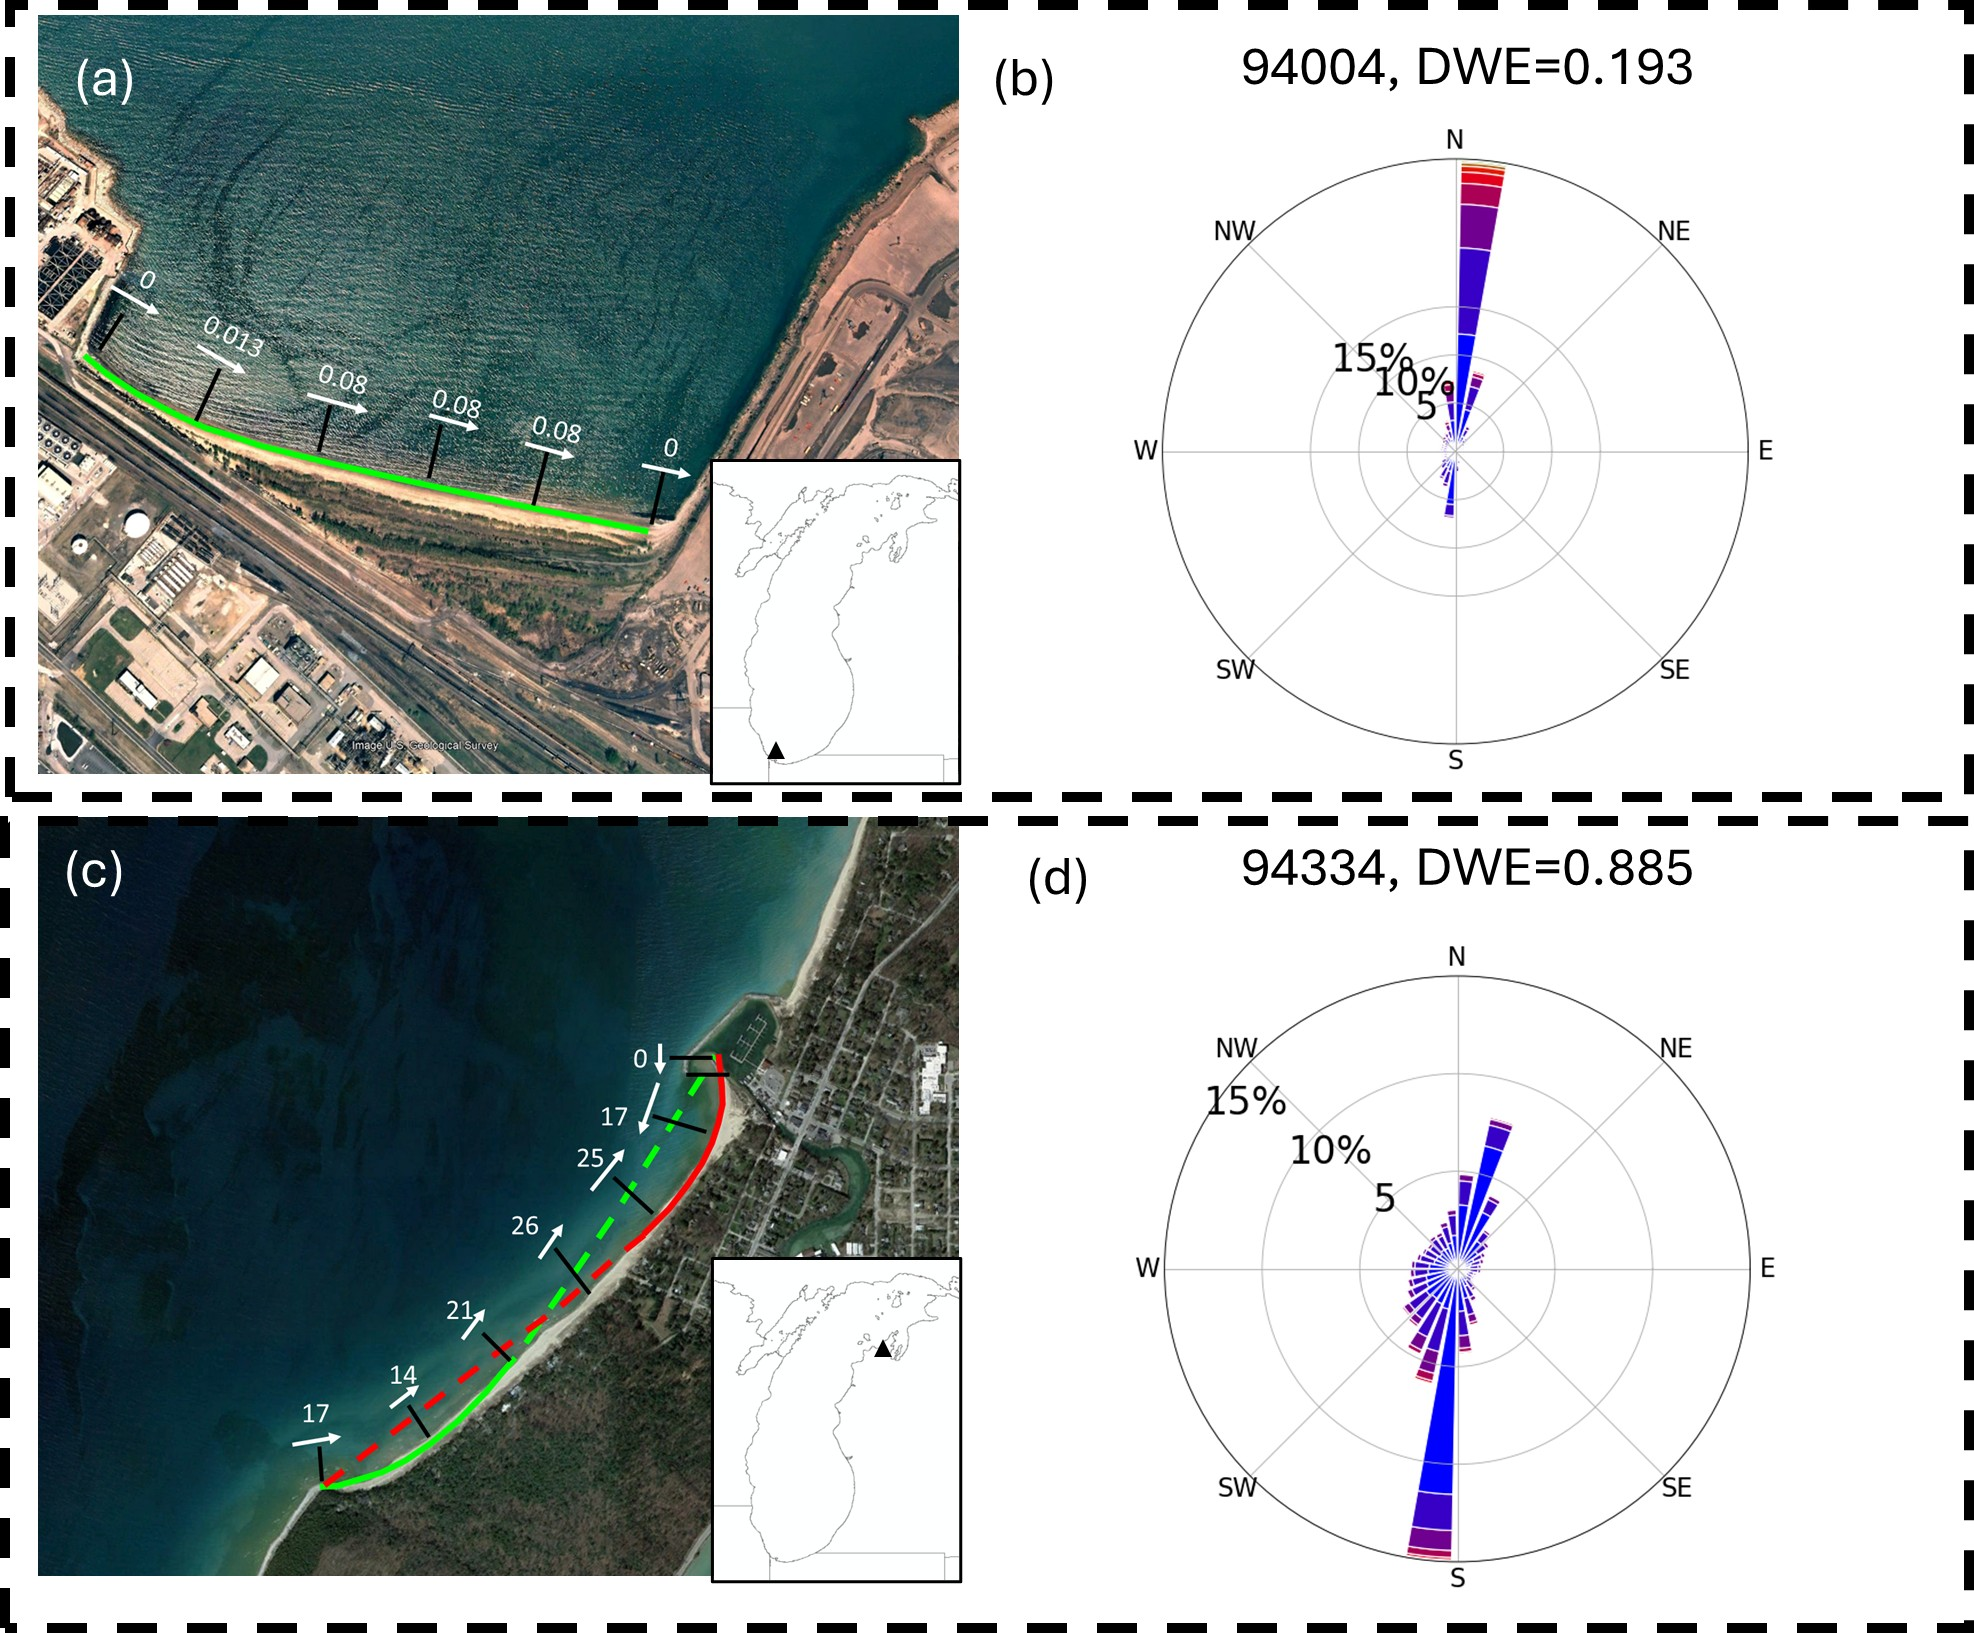
\includegraphics[width=0.8\textwidth]{appendix/resources/figure3-3a.jpg}
  \caption{Wave directionality in Lake Michigan for different DWE thresholds. Wave directionality (red dots are bi-directional and green dots are uni-directional) under three different thresholds: (a) 0.57 (b) 0.65 (c) 0.70. The unit of LST rate is cubic meter per day.}
  \label{fig:fig3.3a}
\end{figure}